\documentclass[12pt,a4paper]{scrartcl}

\usepackage[utf8]{inputenc}
\usepackage[T1]{fontenc}
\usepackage[ngerman]{babel}

\usepackage[pdftex]{graphicx}
\usepackage{latexsym}
\usepackage{amsmath,amssymb,amsthm}
\allowdisplaybreaks
\usepackage{dsfont}
\usepackage{pifont}
\usepackage{nicefrac}
\usepackage{textcomp}
\usepackage{enumitem}
\usepackage{lmodern}

% Abstand obere Blattkante zur Kopfzeile ist 2.54cm - 15mm
\setlength{\topmargin}{-15mm}	   
                  
\numberwithin{equation}{section} 

\newcommand{\C}{\mathbb{C}} % komplexe
\newcommand{\K}{\mathbb{K}} % komplexe
\newcommand{\R}{\mathbb{R}} % reelle
\newcommand{\Q}{\mathbb{Q}} % rationale
\newcommand{\Z}{\mathbb{Z}} % ganze
\newcommand{\N}{\mathbb{N}} % natuerliche
\newcommand{\PP}{\mathbb{P}} % Probability
\newcommand{\E}{\mathcal{E}} % big Epsilon

\numberwithin{equation}{section}%

\theoremstyle{definition}
\newtheorem{exmp}{Example}[section]
\newtheorem{theorem}{Theorem}[section]
\newtheorem{corollary}{Corollary}[theorem]
\newtheorem{lemma}[theorem]{Lemma}
\newtheorem{definition}[theorem]{Definition} 
\newtheorem{proposition}[theorem]{Proposition}

\newtheorem{thm}{Theorem}[section]%
\newtheorem{lem}[thm]{Lemma}%
\newtheorem{satz}[thm]{Satz}%
\newtheorem{prop}[thm]{Proposition}%
\newtheorem{algo}[thm]{Algorithmus}%

\newtheorem{cor}[thm]{Corollary}%
\theoremstyle{definition}
\newtheorem{dfn}[thm]{Definition}%
\newtheorem{rem}[thm]{Remark}%
\newtheorem{com}[thm]{Comment}
\newtheorem{exa}[thm]{Example}%
\newtheorem{bew}[thm]{Beweis}%


\begin{document}
	\pagestyle{empty}

\begin{titlepage}

	
\includegraphics[scale=0.45]{kit-logo.jpg} 
    \vspace*{2cm} 
\begin{center} \large 
    
   Masterthesis
    \vspace*{2cm}

    {\huge External DLA}\\
    \vspace*{2.5cm}

    Tillmann Tristan Bosch
    \vspace*{1.5cm}

    10. March 2020
    \vspace*{3.5cm}


    Supervisor: PD. Dr. Steffen Winter \\[1cm]
    Mathematics Faculty\\[1cm]
	Karlsruhe Institute of Technology
\end{center}
\end{titlepage}

\newpage

\newpage
\phantom \\
\newpage

\tableofcontents %Inhaltsverzeichnis

 	\pagestyle{headings}

\setcounter{page}{1}
\section{Einleitung}
External DLA beschreibt einen stochastischen Prozess, welcher zumindest in ähnlicher Form in natürlichen Prozessen beobachtbar ist. Er ähnelt zum Beispiel der fraktalen Gestalt eines sich kreisförmig ausbreitenden Risses einer Glasscheibe, oder eines Risses eines Kristallfluids wie in LCD Displays in alten Autoradios (siehe Fotos). Er kann auch in Schneeflocken oder in elektrostatischen Anhaftungen an Metallen beobachtet werden. Die Formalisierung solcher Prozesse ist sehr aktuell und die sehr konstruktive Definition erlaubten bisher nur mühsame Folgerungen über Struktur und Verhalten des Prozesses. Wir werden uns Modelle auf $\mathbb{Z}^2$, sowie auf anderen Graphen, darunter auch fraktale Graphen, anschauen, und außerdem versuchen, eine Approximation der bisherigen Definition zu finden, die grundsätzlich handlicher ist und auf einfachere Weise zu Erkenntnissen führt. Wir werden außerdem diese Arbeit mit einigen Python Simulationen begleiten. Der Code ist frei verfügbar auf Github. \\
\\

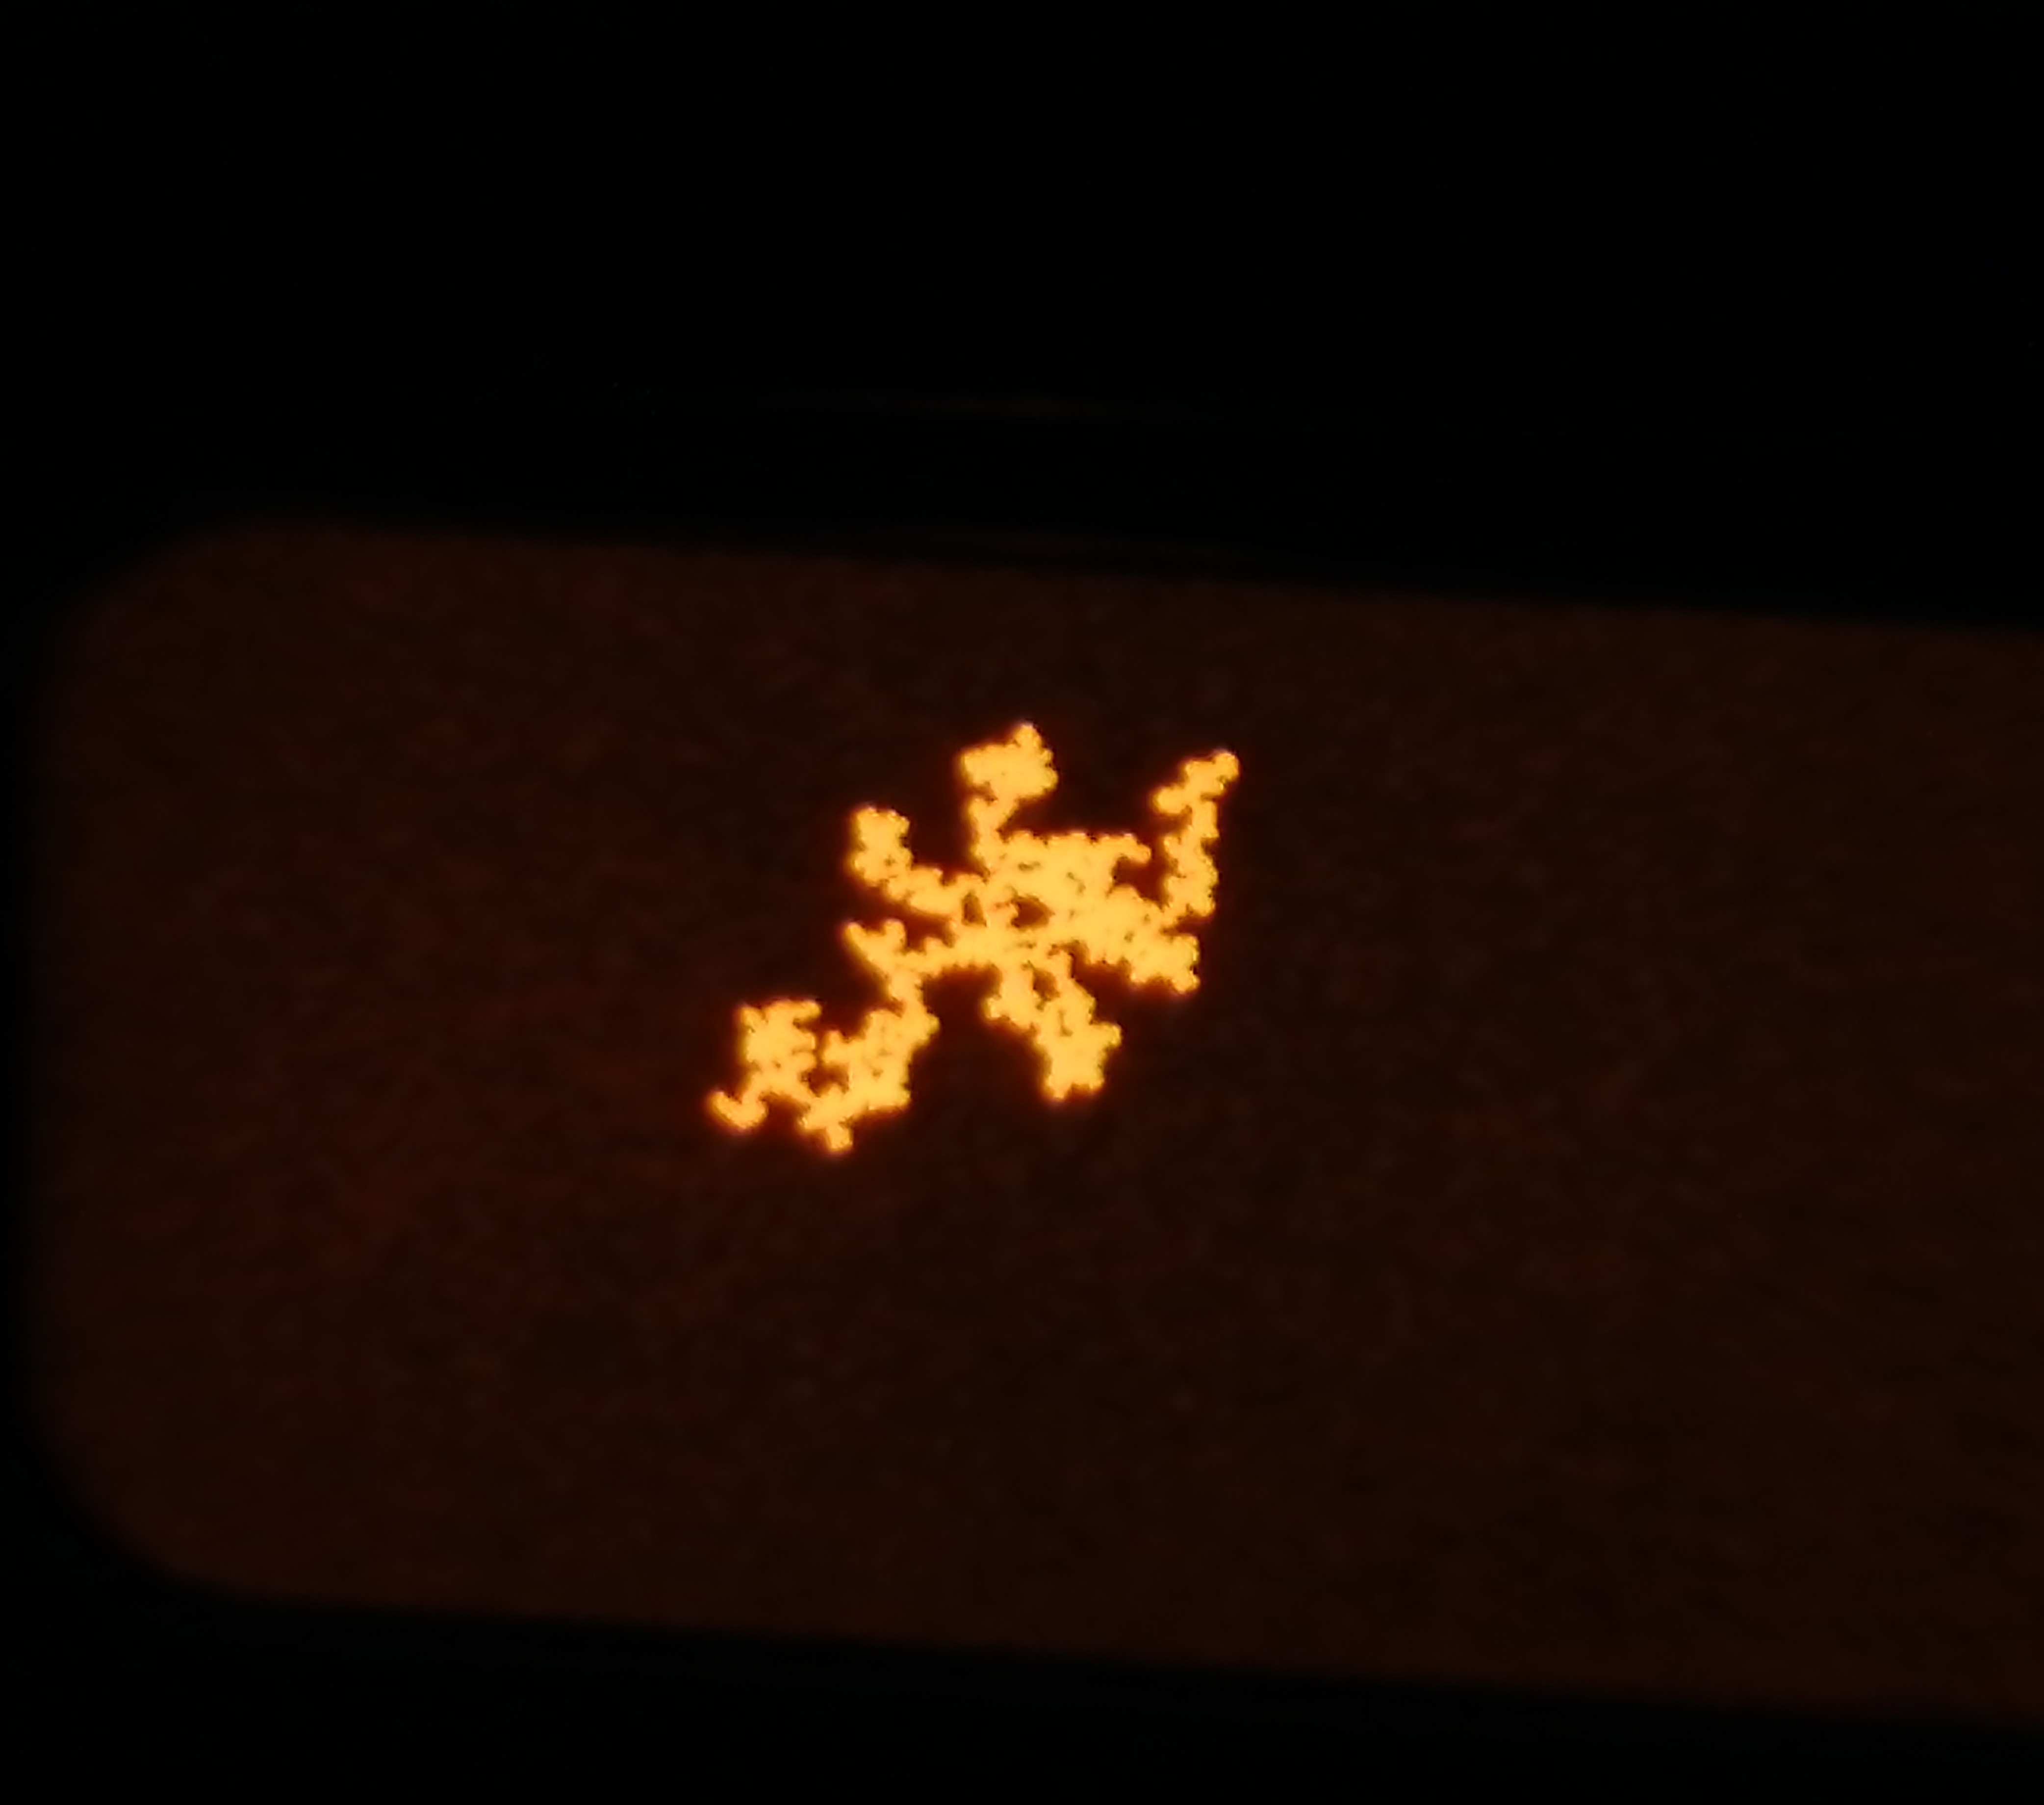
\includegraphics[scale=0.04]{display.jpg} 

\includegraphics[scale=0.091]{display2.jpg} 

\newpage


\section{Preliminaries}

We prepare this script with the following preliminaries. \\
\\
$\boldsymbol{Graphs}.\quad$ Let $G$ be an infinite graph. Denote $deg(x)$ the degree of a vertex $x\in G$. $G$ shall be additionally locally finite, i.e. $deg(x)<\infty$ for all $x\in G$. Let $o\in G$ be a distinguished vertex which we call $origin$ or $root$. Define the distance between two vertices $x,y\in G$ as 
\begin{align*}
	d(x,y):=\min \{n\geq 1\ |\ \exists\ x_1,\dots, x_{n-1}\in G:\ (x,x_1), (x_1,x_2),\dots, (x_{n-1},y) \in E(G)\},
\end{align*}
thus the distance between two vertices is the minimal length of paths connecting the two vertices. For $n\in \mathbb{N}$ and $x\in G$ $balls$ are defined as $B_n(x):=\{y\in G|d(x,y)\leq n\}$, and for the special case $B_n:=B_n(o)$. Let $A\subset G$ a subgraph, then we define the boundary of $A$ as
\begin{align*}
	\partial A := \{y\in G\setminus A\ |\ \exists\ x\in A: (x,y)\in E(G)\}.
\end{align*}

\noindent $\boldsymbol{Random\ Walks}.\quad$ Let $(S_n)_n$ be a random walk on $G$ and denote $\mathbb{P}_x$ the probability measure of the random walk started at $x$. That means precisely 
\begin{align*}
	\mathbb{P}_x(A) := \mathbb{P}_{S_n}(A|S_0=x) = \mathbb{P}(S_n\in A|S_0=x)
\end{align*}
for any subset $A\subset G$. We define the $hitting\ time$ of A as 
\begin{align*}
	T(A) := \min \{n\geq 0\ |\ S_n\in A\},
\end{align*}
and for the special case $T(\{x\})=:T(x)$ for every $x\in G$. The $heat\ kernel$ of the random walk $S_n$ is defined to be 
\begin{align*}
	p_n(x,y):=\mathbb{P}_x(S_n=y)
\end{align*}
and following the $Green\ function$ as 
\begin{align*}
	G(x,y) := \sum_{n\geq 0} p_n(x,y).
\end{align*}
Similarily for a subset $A\subset G$ the $killed$ or $stopped\ Green\ function$ is defined as
\begin{align*}
	G_A(x,y) := \sum_{n\geq 0} \mathbb{P}_x(S_n=y, T(A) > n).
\end{align*} 
\noindent The $hitting\ distribution$ of elements in $A$ with $hitting\ position$ $S_{T(A)}$ is then
\begin{align*}
	H_A(x,y) := p_{T(A)}(x,y),\quad y\in A, 
\end{align*}
and for the special case $x=o$ we define
\begin{align*}
	h_A(y) := H_A(o,y) = \mathbb{P}_o(S_{T(A)}=y),\quad y\in A.
\end{align*}
Thus, $h_A(y)$ is the probability of hitting $A$ for the first time at $y$ starting from $o$. $h_A$ is called the $harmonic\ measure\ (from\ o)$.

\section{Incremental Aggregation}
In this paper we will look at stochastic processes on the set of finite subsets of $\mathbb{Z}^d$, where we start with a one point set at $(0,0)$ and incrementally add a point on the edgeset of the current cluster according to some distribution. What we get is a randomly, point-by-point growing connected cluster which here we will call $\mathit{Incremental\ Aggregation}$. Define 
\begin{align}
	\mathcal{P}_C := \{A\subset \mathbb{Z}^d\ |\ \text{A is finite and connected}\}, 
\end{align}
the set of finite and connected subsets of $\mathbb{Z}^d$. Furthermore we will be interested in distributions on those sets, so for $A\in \mathcal{P}_C$ we define 
\begin{align}
	\mathcal{D}_A:= \{\mu: \mathbb{Z}^d\to [0,1]\ |\ \mu(y) = 0, \forall y\notin A\ \text{and}\ \sum_{y\in A} y = 1 \}.
\end{align}
So every element in $\mathcal{D}_A$ naturally defines a distribution on the elements of $A$. Now we define incremental aggregation as follows.  

\begin{definition}
	Let $\mu=(\mu_A)_{A\in \mathcal{P}_C}$ be a family of distributions with $\mu_A\in \mathcal{D}_A$ for all $A\in \mathcal{P}_C$. $\mathit{Incremental\ Aggregation\ (with\ distribution\ \mu)}$ is a stochastic process $(\mathcal{E}_n)_{n\in{\mathbb{N}_0}}$ which evolves as follows. The process starts with one point $\mathcal{E}_0 = \{(0,0)\}$. Knowing the process $\mathcal{E}_n$ at time $n$, let $y_n$ be a random point on $\partial \mathcal{E}_n\in \mathcal{P}_C$ with distribution
	\begin{align}
		\mathbb{P}(y_n = y\ |\ \mathcal{E}_n) := \mu_{\partial \mathcal{E}_n}(y),\quad y\in \mathbb{Z}^d.
	\end{align}
	We then define $\mathcal{E}_{n+1} := \mathcal{E}_n \cup \{y_n\}$.
\end{definition} 

\begin{rem}
	
\end{rem}

\begin{definition}
	Incremental Aggregation with the harmonic measure $h_A$ as its distribution we define here and is known as $\mathit{Diffusion\ Limited\ Aggregate}$, short $\mathit{DLA}$.
\end{definition}

\newpage

\newpage
\section{External DLA}

External DLA is a model building a sequence of random growing sets $(\mathcal{E}_n)_{n\geq 0}$ starting with one particle $\mathcal{E}_0=\{o\}$ at the origin. At each timestep $n+1$ a new particle starts a random walk $(S_k)_k$ from "far away" (infinity) until it hits the boundary $\partial \mathcal{E}_n$ of the current exting cluster for the first time. The union of this vertex and the already exting cluster then form the new cluster. Lets see the formal definition.

\begin{definition}
	Let $G$ be an infinite graph and $(S_n)_n$ a random walk on it. $External\ DLA$ on $G$ is a Markov chain $(\mathcal{E}_n)_{n\geq 0}$ on finite subsets of $G$ which evolve in the following way. We start with a single vertex at the origin, thus $\mathcal{E}_0 := \{o\}$. Then given the process $\mathcal{E}_n$ at time $n$, let $y_{n+1}$ be a random vertex in $\partial \mathcal{E}_n$ chosen according to the harmonic measure (from infinity) of $\partial \mathcal{E}_n$. Precisely that is
	\begin{align*}
		\mathbb{P}(y_{n+1}=y\ |\ \mathcal{E}_n) = \mu_{\partial \mathcal{E}_n}(y),\quad y\in \partial \mathcal{E}_n.
	\end{align*}
	We then set $\mathcal{E}_{n+1} := \mathcal{E}_n \cup \{y_{n+1}\}$.	
	
\end{definition}

\begin{com}
	Given the definition above, how does a realization of the process mathematcially look like? We start with a constant $\mathcal{E}_0 = \{o\}$. Now we want to realize a vertex $y_1$ in $\partial \mathcal{E}_0$. For this choose $\omega_1\in \Omega$ and realize a random walk $(S(\omega_1)_n)_n$ at $\omega_1$ (starting from infinity). $y_1(\omega_1)$ is the hitting vertex of the random walk and $\partial \mathcal{E}_0$. We can then can set a realization of $\mathcal{E}_1$, which is $\mathcal{E}_1(\omega_1)=\{o,y_1(\omega_1)\}$. 
\end{com}

\newpage


\section{Notizen}

diffusion in fractals: $d_f < d$ (space $\mathbb{Z}^d$)


\newpage


\section{Line Process}

In the following we will look at a process which is the approach of a simple approximation of external DLA. The idea is to let particles move on straight lines coming from infinity and add to the cluster when hitting it. Obviously in most cases particles cannot move completely straight on $\mathbb{Z}^d$. Therefore we will consider points in $\mathbb{Z}^d$ as the centers of unit squares and let the particles move on straight lines in the full plane $\mathbb{R}^d$. We consider the line hitting a point in $\mathbb{Z}^d$ if it cuts its unit square as defined in the following. 

\begin{definition}
	Define 
	\begin{align}
		G_{sq} := \{[k - \frac{1}{2}, k + \frac{1}{2}) \times [l- \frac{1}{2}, l + \frac{1}{2}) \subset \mathbb{R}^2\ |\ k,l \in \mathbb{Z}\}, 
	\end{align} 
	note that $\mathbb{R}^2 = \bigcup_{s\in G_{sq}} s$ and $s_1\cap s_2 = \emptyset$ for all $s_1\neq s_2\in G_{sq}$. The canonical function
	\begin{align}
	sq: \mathbb{Z}^2 \to G_{sq},\quad (k,l)\to [k - \frac{1}{2}, k + \frac{1}{2}) \times [l- \frac{1}{2}, l + \frac{1}{2})
	\end{align}
	is bijective and intuitively identifies points in $\mathbb{Z}^2$ with squares in $\mathbb{R}^2$. In the following when using a point $p\in \mathbb{Z}^2$ it will reference the point in $\mathbb{Z}^2$ or the corresponding square in $\mathbb{R}^2$ respecting the context. This bijection also naturally defines a graph structure on $G_{sq}$, which is two squares $s_1, s_2\in G_{sq}$ form an edge if and only if $sq^{-1}(s_1)$ and $sq^{-1}(s_2)$ form an edge in $G$. We call $L\subset \mathbb{R}^2$ a $line$ if and only if there exist $a,b\in \mathbb{R}^2$ such that $L=\{a+tb\in \mathbb{R}^2\ |\ t\in \mathbb{R}\}$. For the following context we say a line $L$ $hits$ a point $p\in \mathbb{Z}^2$ if and only if $L\cap sq(p) \neq \emptyset$.
	
\end{definition}

BILD Linie durch squares "hitting"\\
Gradenmaß

\begin{definition}
	Similair to the definition of a DLA process we now define a stochastic process $(\epsilon_n)_{n\in \mathbb{N}_0}$ on the set of subsets of $G_{sq}$. We start with $\epsilon_0 =  \{(0,0)\}$. Having the process $\epsilon_n$ after $n$ steps, the next  
\end{definition}




\newpage


\begin{thebibliography}{Lam00}
\thispagestyle{empty}

\bibitem{Henze Skript}
N. Henze.
\emph{Maß und Wahrscheinlichkeitstheorie (Stochastik II)}.
Karlsruher Institut für Technologie, Karlsruhe, 2010

\end{thebibliography}

\newpage
  
\thispagestyle{empty}

\vspace*{8cm}


\section*{Erklärung}

Hiermit versichere ich, dass ich diese Arbeit selbständig verfasst und keine anderen als die angegebenen Quellen und Hilfsmittel benutzt, die wörtlich oder inhaltlich übernommenen Stellen als solche kenntlich gemacht und die Satzung des Karlsruher Instituts für Technologie zur Sicherung guter wissenschaftlicher Praxis in der jeweils gültigen Fassung beachtet habe. \\[2ex] 

\noindent
Karlsruhe, den 10. März 2020\\[5ex] 

\end{document}

